%-----------------------------------------------%
%             filename: skeleton.tex
%-----------------------------------------------%
\documentclass[aps,twocolumn]{revtex4-1}
\usepackage{graphicx}
\usepackage{ifpdf}
\ifpdf
	\usepackage[backref]{hyperref}
	%\usepackage[backref,pageanchor=true,plainpages=false, pdfpagelabels,bookmarks,bookmarksnumbered]	{hyperref}
\else
\fi

\usepackage{crs}

% see http://goo.gl/5Fo27
\newtoggle{thmsty}
%\toggletrue{thmsty}
\togglefalse{thmsty}

% see http://goo.gl/7jLZ9
\makeatletter
\newlength \figwidth
\if@twocolumn
  \setlength \figwidth {0.8\columnwidth}
\else
  \setlength \figwidth {0.5\textwidth}
\fi
\makeatother

\begin{document} 

\title{\bf Intrinsic information representation in biological systems}

\author{a1$^{1}$, a2$^{1}$, a3$^{1}$, a4$^{1,2,3}$}

\affiliation{$^1$Department of Systems and Computational Biology,\\ $^2$Dominick P. Purpura Department of Neuroscience, \\ $^3$Department of Pathology, Albert Einstein College of Medicine, 1301 Morris Park Ave, Bronx, NY 10461, USA}

\date{\today}
\begin{abstract}
One of the most important aspects of advancing theory in biology is the development of a constructed language that can be explicitly and precisely defined thereby supporting communication, computer-based knowledge representation, and hypothesis-generating thought. Such a language should itself be evolvable and support flexible abstractions that enable the unification and compression of redundant information via the expression of principles of invariance. It would be useful for such a language to be formally specified prior to or in concert with the development of a computational implementation that may support complementary organization of autonomously linked data. We propose the specialization of a language originally developed in a mathematical context that apparently meets these criteria. We argue for this choice, not from a mathematical perspective but, by providing an example of the way in which this language enables precise qualitative reasoning and flexible methods of abstraction with respect to integrating biological information in a manner that would, ideally, be analogous to the way in which information is integrated by biological systems themselves. Enabling lossless compression and representation of synthetic knowledge about biological systems, in addition to raw biological data, is necessary for understanding in the context of limited cognitive and other computational resources.
\end{abstract}

\maketitle

\tableofcontents

\section{Introduction}

\begin{figure*}
\noindent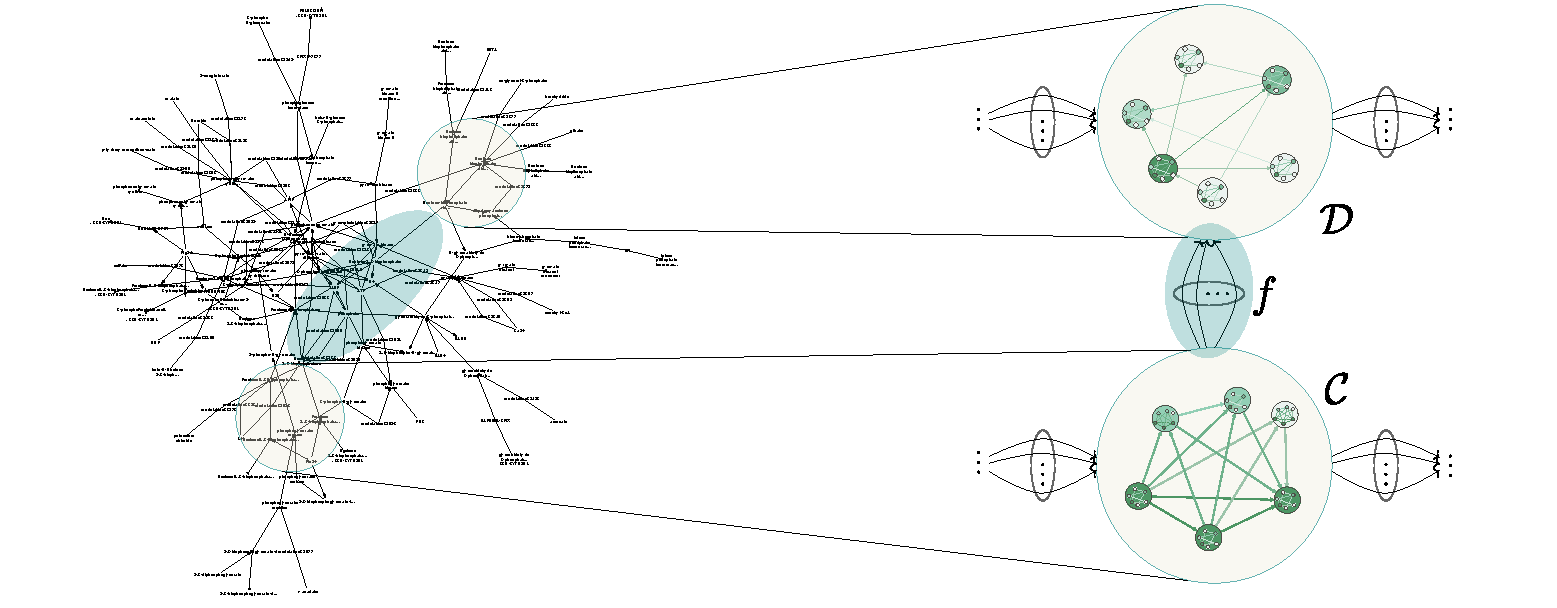
\includegraphics[width=1.8\columnwidth]{fig/biograph.pdf}
\caption{Particular features of interaction networks underlying biological systems can be abstracted as graphs of some type with morphisms translating structure between them.}
\label{fig:biograph}
\end{figure*}

The development of a formal language for modeling biological systems was suggested by Joseph Woodger in collaboration with the developmental biologist Conrad Waddington and the logician Alfred Tarski as early as 1937 \cite{Woodger1937,Woodger1951,Woodger1952,Woodger1952a}. At that time it was perhaps difficult to understand how such a language could be put to use. Today we have tools that could enable the use of such a language: namely 1) computational machines to automate the details of routine transformations within the language and 2) large, accessible, growing repositories of biological data. Though we have access to necessary infrastructure, we lack such a language suggested by Woodger and others throughout the course of the 20th century as we have continued to rely on natural language heuristics to communicate and reason about biological systems.

Category theory \cite{Lane1985,Lane1998,MacLane1992,Lawvere1997,Lawvere2003,Awodey2006} is a language that has been suggested since Woodger to provide a framework for representing and reasoning about biological systems \cite{GOGUEN1979,Ehresmann2007,Louie2009}. What is immediately useful about this language from the perspective of biology is that it presents as primitive the notion of transformation or interaction between objects. In fact, from this point of view, a defining characteristic of any entity (e.g. a protein, cell, organism, or population) is structural: the set of relationships between it and other entities under consideration. Intrinsic properties are taken into account implicitly in this framework since the possible set of relationships between any object and any other is constrained by the nature of its intrinsic properties. 

What may be less obvious at first meeting is the way in which concepts from category theory, especially with regard to its interface with logic and geometry \cite{MacLane1992,Jacobs1998}, enable the formulation of what might be viewed as a framework for explaining the nature and development of so-called \emph{emergent properties} of systems that are able to represent information in molecular terms at their base, but build upon this to generate the capacity to process information at higher levels of organization as well. We note that the existence of {\it levels of organization} that may have come into existence during the evolutionary process thus far, although common in various informal taxonomic systems used in biology, is a hypothesis that we hope to render verifiable in the long term through the introduction of a language capable of making predictions that could help distinguish the case in which there is from that in which there is not justification to reify the conceptual levels of organization that have been introduced to organize biological knowledge. The concept of separation of spatio-temporal scales, which is used to justify the consideration of one level of organization at a time in the biological model-building process \cite{Gunawardena2012,Karr2012}, may make it impossible to explain evolutionary processes that transcend such levels of organization providing one justification to our search for a language that can support model-building that does not require such approximations. The expression discussed here is general enough that it can be equally well applied to the consideration of relationships between any levels of biological organization assuming that any at all exist. Of course, it will need to be further specialized to be of use in specific contexts. However, the unity deriving from the judicious definition of underlying categorical concepts along the way is precisely the type of abstraction that we argue is necessary to enable conceptual compression of biological information and thereby improve our capacity to communicate and synthesize existing and future knowledge about biological systems.

Here we explain the concepts from category theory necessary to understand the way in which interacting objects at one level of organization (e.g. molecules) can produce phenomena that would themselves be identifiable as derived objects (e.g. cells) that justify the very conceptualization of a \emph{level of organization} in the first instance. Here we focus exclusively on defining the boundary conditions relating levels (e.g. molecules and cells or cells and multicellular organisms) of organization, which are necessary to understand in the course of defining a dynamical system that could model the \emph{evolution} of such. What results is a refinement of the concept of the levels of organization that are ubiquitously employed in biology and examples of which are used so far only heuristically as guides to pre-existing intuition. Understanding how to integrate information regarding biological processes across such levels of organization is fundamental to the understanding of complex phenotypes and the associated set of contingencies necessary to account for in methods that may be targeted at controlling or otherwise manipulating them.

[ Note that biological systems are concretely represented as graphs of some kind and all the letters representing categories can be specialized to categories of graphs of some kind ]

\begin{quotation}
{\it One such idea, which underlies everything in this book, is the concept
of genomically encoded information processing. To return to my metaphor above,
this is like the geological basis of the landscape. In my view, cis-regulatory information processing, and information processing at the gene regulatory network circuit level, are the real secret of animal development. Probably the appearance of genomic regulatory systems capable of information processing is what made animal evolution possible.} -Eric H. Davidson \cite{Davidson2006a}
\end{quotation}

\section{Intrinsic operationalism in biological systems}
\subsection{System-environment duality}
Distinction between biological systems or some components thereof and the environments within which they are embedded is implied in models of such systems. This distinction is useful in many contexts, but the boundary between a biological system and its environment is dependent upon the level of resolution of the \emph{model and modeler} independent of its relationship to properties of the biological system itself \cite{Fontana1996}. In this light, it is desirable to develop a model of biological systems that supports variation of this boundary without requiring complete reconfiguration of the model. Constructing a framework for such models requires the determination, unification, and incorporation of abstract features of biological systems that are invariant across levels of organization from molecules to cells, organisms, populations, communities, ecosystems and more fine-grained levels of resolution that likely lie between these broadly and imprecisely defined perspectives one can take with regard to representing biological systems.

\subsection{General coherence constraints for intrinsic biological information representation}
The use of categorical adjunctions to model intrinsic information representation in biological systems has been suggested \cite{GOGUEN1979,Ellerman2005}, but these efforts have yet to be incorporated into more detailed theories. This may be in part a result of the difficulty in specifying the appropriate level of abstraction at which a precise metaphor can be developed between collections of interacting biological entities and a particular type of mathematical structure. We begin here by developing the prerequisite definitions to explain why the transformation of biological information is naturally represented as a pair of adjoint functors in the context of category theory. A relevant piece of intuition to associate to what follows is that any interaction between biological entities is, minimally, a dyadic relationship wherein contingencies associated to other interactions of each of the participants establishes prerequisite potential value to high fidelity transmission and representation of information regarding the state of other collections of spatio-temporally distant interactions. The participants in such a dyadic interaction are modelled as categories because each may represent an underlying arbitrarily complicated collection of interactions that are necessary for the very existence of the interface implicit to any interaction.

\iftoggle{thmsty}{
\begin{definition}
\label{definition-category}
}{}
A {\it category} $\mathcal{C}$ is:
\begin{enumerate}
\item A set of objects $\Ob(\mathcal{C})$.
\item For each pair $x, y \in \Ob(\mathcal{C})$ a set of morphisms
$\Mor_\mathcal{C}(x, y)$.
\item For each triple $x, y, z\in \Ob(\mathcal{C})$ a composition
map $ \Mor_\mathcal{C}(y, z) \times \Mor_\mathcal{C}(x, y)
\to \Mor_\mathcal{C}(x, z) $, denoted $(\phi, \psi) \mapsto
\phi \circ \psi$.
\end{enumerate}
Such that these constraints are satisfied:
\begin{enumerate}
\item For every element $x\in \Ob(\mathcal{C})$ there exists a
morphism $\text{id}_x\in \Mor_\mathcal{C}(x, x)$ such that
$\text{id}_x \circ \phi = \phi$ and $\psi \circ \text{id}_x = \psi $.
\item Composition is associative, i.e., $(\phi \circ \psi) \circ \chi =
\phi \circ ( \psi \circ \chi)$.
\end{enumerate}
\iftoggle{thmsty}{
\end{definition}
}

\iftoggle{thmsty}{
\begin{definition}
\label{definition-functor}
}{}
A {\it functor} $F : \mathcal{A} \to \mathcal{B}$
between two categories $\mathcal{A}, \mathcal{B}$ is:
\begin{enumerate}
\item A map $F : \Ob(\mathcal{A}) \to \Ob(\mathcal{B})$.
\item For every $x, y \in \Ob(\mathcal{A})$ a map
$F : \Mor_\mathcal{A}(x, y) \to \Mor_\mathcal{B}(F(x), F(y))$,
denoted $\phi \mapsto F(\phi)$.
\end{enumerate}
These data should be compatible with composition and identity morphisms
in the following manner: $F(\phi \circ \psi) =
F(\phi) \circ F(\psi)$ for a composable pair $(\phi, \psi)$ of
morphisms of $\mathcal{A}$ and $F(\text{id}_x) = \text{id}_{F(x)}$.
\iftoggle{thmsty}{
\end{definition}
}

\iftoggle{thmsty}{
\begin{definition}
\label{definition-transformation-functors}
}{}
Let $F, G : \mathcal{A} \to \mathcal{B}$ be functors.
A {\it natural transformation}, or a {\it morphism of functors}
$t : F \to G$, is a collection $\{t_x\}_{x\in \Ob(\mathcal{A})}$
such that
\begin{enumerate}
\item $t_x : F(x) \to G(x)$ is a morphism in the category $\mathcal{B}$, and
\item for every morphism $\phi : x \to y$ of $\mathcal{A}$ the following
diagram is commutative
$$
\xymatrix{
F(x) \ar[r]^{t_x} \ar[d]_{F(\phi)} & G(x) \ar[d]^{G(\phi)} \\
F(y) \ar[r]^{t_y} & G(y) }
$$
\end{enumerate}
\iftoggle{thmsty}{
\end{definition}
}

We can define a category having functors as objects and natural transformations as morphisms, which is called a functor category, by recognizing that every functor $F$ comes with the {\it identity} transformation $\text{id}_F : F \to F$. In addition, given a morphism of
functors $t : F \to G$ and a morphism of functors $s : E \to F$
then the {\it composition} $t \circ s$ is defined by the rule
$$
(t \circ s)_x = t_x \circ s_x : E(x) \to G(x)
$$
for $x \in \Ob(\mathcal{A})$.
This is a morphism of functors
from $E$ to $G$.
Thus, given categories
$\mathcal{A}$ and $\mathcal{B}$ we obtain the category of functors between $\mathcal{A}$ and
$\mathcal{B}$.

\iftoggle{thmsty}{
\begin{definition}
\label{definition-equivalence-categories}
}{}
An {\it equivalence of categories}
$F : \mathcal{A} \to \mathcal{B}$ is a functor such that there
exists a functor $G : \mathcal{B} \to \mathcal{A}$ such that
the compositions $F \circ G$ and $G \circ F$ are isomorphic to the
identity functors $\text{id}_\mathcal{B}$,
respectively $\text{id}_\mathcal{A}$.
In this case we say that $G$ is a {\it quasi-inverse} to $F$.
\iftoggle{thmsty}{
\end{definition}
}

\iftoggle{thmsty}{
\begin{definition}
\label{definition-adjoint}
}{}
Let $\mathcal{C}$, $\mathcal{D}$ be categories.
Let $u : \mathcal{C} \to \mathcal{D}$ and
$v : \mathcal{D} \to \mathcal{C}$ be functors.
We say that $u$ is a {\it left adjoint} of $v$ or that
$v$ is a {\it right adjoint} to $u$, written $u \dashv v$, if there are bijections
$$
\phi_{X,Y}:\Mor_\mathcal{D}(u(X), Y)
\simeq
\Mor_\mathcal{C}(X, v(Y))
$$
functorial in $X \in \Ob(\mathcal{C})$, and
$Y \in \Ob(\mathcal{D})$.
\iftoggle{thmsty}{
\end{definition}
}

$F \dashv G$ is thus equivalent to the statement $\phi_{-,-}:b_{(-)} \cong b^{(-)}$ (see Appendix \ref{app:CatTh}). In this framework, information encoding/decoding is an asymmetric process that can only be accomplished without loss of information in one direction: objects of $\cD$ can be encoded into objects of $\cC$ and decoded into objects of $\cD$ but, in general, proceeding in the opposite order may result in loss of information. This asymmetry is clarified by consideration of the unit and counit morphisms of the adjunction.

\iftoggle{thmsty}{
\begin{definition}
\label{definition-unit}
}{}
Consider the identity morphism $1_{Fc} \in \Mor_{\cD}(Fc,Fc)$. The adjoint transpose of $1_{Fc}$ is the {\it unit} morphism at $c$
$$
\phi_{c,Fc}(1_{Fc})=1_{Fc}^*=\eta_c: c \rightarrow GFc
$$
where $\eta_c \in \Mor_{\cC^{opp}}(c,GFc)$, which, when taken to be natural in $c \in \Ob(\cC^{opp})$, gives the natural transformation
$$
\eta : 1_{\cC^{opp}} \Rightarrow GF
$$
\iftoggle{thmsty}{
\end{definition}
}

\iftoggle{thmsty}{
\begin{definition}
\label{definition-counit}
}{}
Consider the identity morphism $1_{Gd} \in \Mor_{\cC^{opp}}(Gd,Gd)$. The adjoint transpose of $1_{Gd}$ is the {\it counit} morphism at $d$
$$
\phi_{Gd,d}^{-1}(1_{Gd})=1_{Gd}^*=\epsilon_d: FGd \rightarrow d
$$
where $\epsilon_d \in \Mor_{\cD}(d,FGd)$, which, when natural in $d$, gives the natural transformation
$$
\epsilon: FG \Rightarrow 1_{\cD}
$$
\iftoggle{thmsty}{
\end{definition}
}

The composite encoding inspection functor 
$$
b_{(-)} \circ G(-): \cD \rightarrow \cC^{opp} \rightarrow \textit{Sets}
$$
that specifies a set of morphisms in $\cD$ from the perspective of $\cC^{opp}$ is represented by the pair $(F,\eta)$. Likewise, the composite decoding inspection functor 
$$
b^{(-)} \circ F(-): \cC^{opp} \rightarrow \cD \rightarrow \textit{Sets}
$$
that specifies a set of morphisms in $\cC^{opp}$ from the perspective of $\cD$ is represented by the pair $(G,\epsilon)$. Figure \ref{fig:adjunction} summarizes features of the information encoding-decoding adjunction between $F$ and $G$.

\begin{figure}
\noindent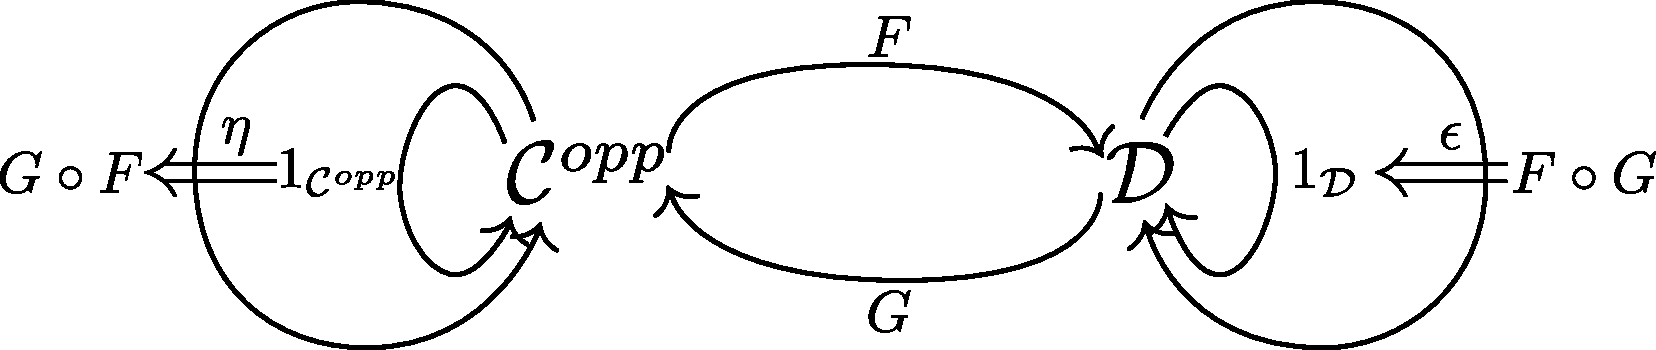
\includegraphics[width=0.9\columnwidth]{fig/adjunction.pdf}
\caption{The adjoint relationship between functors $F \dashv G$ with unit $\eta$ and counit $\epsilon$ natural transformations. The asymmetry in the encoding-decoding relationship indicates that $FG \cD$ can be translated back into the original terms of $\cD$ whereas $GF \cC^{opp}$ cannot be translated back into the original terms of $\cC^{opp}$.}
\label{fig:adjunction}
\end{figure}

The asymmetry of the adjunction can be dispensed with if the unit and counit natural transformations are in fact natural isomorphisms $\eta: 1_{\cC^{opp}} \cong GF$ and $\epsilon: FG \cong 1_{\cD}$. In any limit in which this is the case the adjunction $F \dashv G$ gives an equivalence of categories $\cC^{opp} = \cD$ and the information encoding-decoding process becomes bidirectionally exact.

\subsection{Measurement processes intrinsic to biological systems}
The perspective taken here seeks to abstract from the fundamental relationship between algebraic structures and geometric state spaces that enables translation between them in certain cases \cite{Nestruev2002}. The significance of this perspective is in its capacity to address an important issue that arises in the process of constructing models of biological systems. It is conventional to assume that the geometry of the state space in dynamical models of biological systems is invariantly Euclidean leading to the specification of models of biological systems as a system of ordinary differential equations or the flow of a vector field on a Euclidean manifold, colloquially written as something similar to
$$
\frac{d \vec{x}}{dt} = V(\vec{x}),
$$ 
where $\vec{x}$ is a vector of state variables upon which $V$ is a function specifying a vector field that, for each variable, may be a function of all specified state variables. This framework requires generalization to approach accurate representation of biological systems, which are evolvable. Presumably, the geometry of the state space is not fixed {\it a priori} and is itself constructed as part of the intrinsic dynamics intuitively associated to current understanding of biological systems \cite{Fontana1994,Fontana1996}. In this light, we need to explicitly consider the process by which a state space is intrinsically constructed in the context of developing a theoretical framework for constructing models of biological systems. This can be accomplished within a framework of {\it intrinsic operationalism} \cite{Bridgman1927} that begins with an abstract accounting of measurements that biological entities may perform upon one another leading to the view of morphisms in a category as specifying a measurement process in which the structure of a biological entity is measured in terms of the structure of another \cite{Rosen1978}.
 
At any level of organization, for example in the case of protein-protein interactions \cite{Johnson2010a, Heo2011}, there are interactions that do not provide stable channels for information flow or may poison otherwise stable channels resulting in the appearance of fundamental randomness at the population level. At another extreme, interactions that do support information flow at the population level culminate in robust correlations that may in turn impinge as a selective filter for a particular type of information flow in another connected, but potentially distal, interaction. The space spanning these relative extremes is embodied in structure preserving transformations between objects in a category where the domain object is viewed as an observable and the codomain object is viewed as representing the result of an intrinsic measurement. Of course, these objects may themselves be represented by categories or some higher-order algebraic structure in which the notion of structure preservation implies important subtleties, but the interpretation of a process in which observables take values according to measurements is invariant.
From this perspective, what is necessary to characterize any biological entity is precisely a mechanism for determining the set of interactions in which it participates from the point of view of any other entity with which it interacts. This simple principle has a precise formulation in category theory in terms of {\it Yoneda's lemma}.

\iftoggle{thmsty}{
\begin{definition}
\label{lemma-yoneda}
}{}
Given a category $\cC$, for $c,c' \in \Ob(\cC)$ and $h_{c},h_{c'} \in \Ob(\textit{Sets}^{\cC})$, the {\it covariant Yoneda lemma} states that the set of natural transformations between copresheaves $Nat_{\textit{Sets}^{\cC}}(h_{c'},h_c)$ is isomorphic to $h_{c}(c')=Mor_{\cC}(c,c')$ and natural in $c$ and $c'$:
$$
Nat_{\textit{Sets}^{\cC}}(h_{c'},h_c) \cong Mor_{\cC}(c,c')
$$
Dually, for $h^{c},h^{c'} \in \Ob(\textit{Sets}^{\cC^{opp}})$ the {\it contravariant Yoneda lemma} states that the set of natural transformations between presheaves $Nat_{\textit{Sets}^{\cC^{opp}}}(h^{c},h^{c'})$ is isomorphic to $h^{c'}(c)=Mor_{\cC^{opp}}(c,c')$ and natural in $c$ and $c'$:
$$
Nat_{\textit{Sets}^{\cC^{opp}}}(h^{c},h^{c'}) \cong Mor_{\cC^{opp}}(c,c')
$$
\iftoggle{thmsty}{
\end{definition}
}

The covariant form of Yoneda's lemma in the reverse direction from morphisms to natural transformations implies that if we have an intrinsic measurement procedure $f:c \rightarrow c' \in Mor(\cC)$  where an observable $c$ takes values in $c'$ as the result of an interaction between $c$ and $c'$ then we have an associated natural transformation between the functors represented by $c'$ and $c$, $\xi^{c'}_{c} : h_{c'} \Rightarrow h_c$. 
This relationship has two important meanings. The first is that all of the information implicit in a particular biological entity can be expressed in terms of the set of intrinsic measurement procedures to which it is subjected in interactions with all other biological entities, which is formalized in terms of the functor that it represents $h_c \equiv hom(c,-)$, being a variable set of morphisms parametrized by all other biological entities within the category of such. The second is that if two biological entities interact with all others in equivalent ways, then this will be identified according to the Yoneda lemma by the existence of a natural isomorphism between the functors represented by each.

Depending upon the specific nature of the category modelling biological entities, the functor $h_c$ can be endowed with a geometric interpretation. For example, the evaluation of $h_c$ from the perspective of any $c' \in \Ob(\cC)$ can be taken to represent the set of states within a geometric space that represent $c$ in terms of $c'$ under all possible measurement procedures acting on $c$. Dually, evaluation of the functor $h^c$ from the perspective of any $c' \in \Ob(\cC)$ can be taken to determine all the points specifying measurement values in terms of $c$ which together determine the structure of the state space represented by $c$. In cases where the objects of such a category have sufficient structure, the intuitive security provided by the association between geometry and visualizability is illusory because the only known methods of interrogation of such complicated objects are algebraic. The geometric semantics are nevertheless helpful in the context of explaining the modelling framework.

\section{A topological framework for biological information}

\subsection{Hierarchical biological information representation}

From the perspective of intrinsic operationalism described thus far, the components of biological systems take on the role of the measurements they are capable of performing on and representing in terms of one another. Collections of interacting biological entities can also perform measurements on other collections and it is necessary to establish in our modeling framework a method for representing the way in which collections of interactions can be woven together to produce higher-order structures. Although this choice may be generalized in the future, as a first approximation, we qualitatively associate algebraic rings, which abstractly support concepts of addition and multiplication of measurements fundamental to biological systems \cite{Houle2011}, to the relatively primitive biological entities under consideration that provide a {\it local} description with respect to a {\it global} structure which may be represented by a composite ring of observables that can be constructed by potentially integrating components from each ring defined locally. This perspective suggests the capacity to both deconstruct and resynthesize composite systems in terms of locally and globally defined rings.

The approach outlined above can, in principle, be iterated over multiple local-global transitions where in ascending from bottom to top global objects and the associated measurements they are capable of performing in terms of one another become local objects when the perspective is shifted to the next level of organization. This capacity will be taken advantage of to define a structural condition characterizing the occurrence of a so-called major transition in evolution \cite{MaynardSmith1995,Okasha2006,Calcott2011}. For now, in order to describe the generic relationship between one collection of local entities and another collection of global entities that are composite constructions upon the collection of local entities we first construct a category for each of the local and global levels of interaction, $\mathcal{L}_0$ and $\mathcal{L}_1$, respectively. In general, all the structure in $\mathcal{L}_0$ may be recapitulated in $\mathcal{L}_1$ but not necessarily conversely. In the context of categories of rings the representable functors $h_r$ and $h^r$ where $r \in \Ob(\textit{Rings})$ can be referred to as spectrum functors.

%[[[[[[[[[[[[[[[It might be appropriate to develop the connection to von Neumann algebras, which attempt to generalize $C^*$-algebras by considering general rings of operators and were referred to as such by von Neumann. In addition \cite{Heunen2009} has developed the geometric logic of $C^*$-algebras demonstrating how a state space can be constructed from algebras of observables.]]]]]]]]]]]]]]]

%\subsection{Intrinsic perspectives on biological information representation}

The relationship between local and global biological information representation in the categories $\mathcal{L}_0$ and $\mathcal{L}_1$. We can construct a method for relating local and global biological information contained in these two categories. We have previously defined the Yoneda embedding for an arbitrary category, which we specialize to the case of $\mathcal{L}_0$ as $PSh: \mathcal{L}_0 \rightarrow \textit{Sets}^{\mathcal{L}_0^{opp}}$. We abstractly define a functor to be constructed $A:\mathcal{L}_0 \rightarrow \mathcal{L}_1$ that assigns representations of global information and morphisms that preserve the structure between them to those of local information with respect to a biological system.  Similarly, the functor $R: \mathcal{L}_1 \rightarrow \textit{Sets}^{\mathcal{L}_0^{opp}}$ assigns presheaves on $\mathcal{L}_0$ to the composite information structures in $\mathcal{L}_1$ and $L$ acts conversely. The categories of local and global information representation and the functors enabling partial translation between them is summarized in Figure \ref{fig:ascent}.

\begin{figure}
\noindent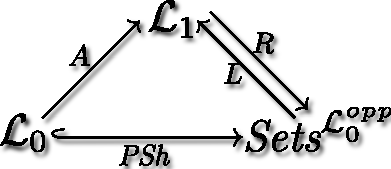
\includegraphics[width=0.5\columnwidth]{fig/ascent.pdf}
\caption{A framework for the construction of a mechanism of local-global translation of biological information. $\mathcal{L}_0$ and $\mathcal{L}_1$ are respectively the categories of relatively local and global biological information structures. The Yoneda embedding functor $PSh$ is already concrete and constructs the presheaf functor category on $\mathcal{L}_0$. The functors $A$, $R$, and $L$ are initially defined abstractly and subsequently constructed.}
\label{fig:ascent}
\end{figure}

In order to construct the functor $L$, we need to explain the relationship between objects in the category of presheaves and the representable functors from their underlying category.

\iftoggle{thmsty}{
\begin{definition}
\label{definition-category-of-elements}
}{}
For any category $\mathcal{C}$, index category $J$, and functor $A:J \rightarrow \cC$, every $P \in \Ob(\textit{Sets}^{\cC^{opp}})$ is a colimit of $\cC$-representable functors
$$
\lim_{\overrightarrow{j \in J}} PSh A_j \cong P.
$$
There is a canonical choice for $J$ and $A$ such that
$$
\lim_{\rightarrow{J}} PSh \circ A \cong P.
$$
The unique index category $J$ is called the {\it category of elements} of the presheaf $P$ and is denoted
$$
\int_{\cC} P.
$$
The objects of $\int_{\cC} P$ are pairs $(C,x)$ where $C \in \Ob(\cC)$ and $x \in PC$. The morphisms are triples $(g,(C',x'),(C,x))$ where $g:(C',x') \rightarrow (C,x)$ derives from $g: C' \rightarrow C \in \Mor(\cC)$ and these satisfy the condition
$$
P(g)(x)=x'.
$$
There is also a projection functor that recovers structure in $\cC$ from the category of elements of $P$
$$
\pi : \int_{\cC} P \rightarrow \cC
$$
defined on objects and morphisms of the category of elements of $P$ respectively as $\pi(C,x)=C$ and $\pi (g,(C',x'),(C,x)) = g$.
\iftoggle{thmsty}{
\end{definition}
}

The category of elements of a presheaf functor is depicted schematically in figure \ref{fig:catofel}. Colimits over the category of elements of a presheaf are used in the construction of the functors $R$ and $L$ suggested in figure \ref{fig:ascent}.

\iftoggle{thmsty}{
\begin{theorem}
\label{theorem-cocompletion-adjunction}
}{}
Consider $\mathcal{L}_0$ a small category, $\mathcal{L}_1$ is a cocomplete category, and a functor $A : \mathcal{L}_0 \rightarrow \mathcal{L}_1$. Then we can construct a pair of adjoint functors $L \dashv R$ between $\mathcal{L}_1$ and $\textit{Sets}^{\mathcal{L}_0^{opp}}$ such that $L: \textit{Sets}^{\mathcal{L}_0^{opp}} \rightarrow \mathcal{L}_1 :R$ where $L$ and $R$ are defined componentwise as
\begin{eqnarray}
R(L_1) &:& L_0 \mapsto Mor_{\mathcal{L}_1}(A(L_0),L_1),\\
L(P) &=& Colim \left( \int P \xrightarrow{\pi} \mathcal{L}_0 \xrightarrow{A} \mathcal{L}_1 \right) .
\end{eqnarray}
\iftoggle{thmsty}{
\end{theorem}
}

\iftoggle{thmsty}{
\begin{proof}
\label{proof-cocompletion-adjunction}
}{}
A natural transformation can be constructed $\tau : P \rightarrow R(L_1)$ by defining it on components as set functions parameterized by $L_0 \in \Ob(\mathcal{L}_0)$
$$
\tau_{L_0} : P(L_0) \rightarrow Mor_{\mathcal{L}_1}(A(L_0),L_1)
$$
which is natural in $C$ according to the commutativity of the diagram
$$
\xymatrix{
P(L_0) \ar[r]^-{\tau_{L_0}} \ar[d]_{P(u)} & Mor_{\mathcal{L}_1}(A(L_0),L_1) \ar[d]^{A(u)^*} \\
P(L'_0) \ar[r]^-{\tau_{L'_0}} & Mor_{\mathcal{L}_1}(A(L'_0),L_1) }
$$
for all $u:L'_0 \rightarrow L_0 \in \Mor(\mathcal{L}_0)$. $\tau$ is also determined by a family of morphisms in $\Mor(\mathcal{L}_1)$ by
$$
\{ \tau_{L_0}(x):A(L_0) \rightarrow L_1 \}_{(L_0,x)}
$$
indexed by objects $(L_0,x)$ of the category of elements $\int P$. This construction is natural in objects $(L_0,x)$ in the sense that the diagram
$$
\xymatrix{
A(L_0) \ar@{=}[r] \ar[dd]_{A(u)} & A\pi(L_0,x) \ar[rd]^{\tau_{L_0}(x)} \ar[dd]^{u_*} & \\
& & L_1 \\
A(L'_0) \ar@{=}[r] & A\pi(L'_0,x') \ar[ru]_{\tau_{L'_0}(x')} &
}
$$
commutes for each morphism $u$. There is thus a bijection
$$
Nat(P,R(L_1)) \cong Mor_{L_1}(LP,L_1),
$$
which is natural in both $P$ and $L_1$ demonstrating the adjoint relationship $L \dashv R$. The functor $L$ is unique for a given $A$ and all functors $A$ from a small category $\mathcal{L}_0$ to a cocomplete category $\mathcal{L}_1$ factor through the Yoneda embedding $PSh$. The Yoneda embedding is thus the universal method of appending colimits to a small category as suggested by the diagram
$$
\xymatrix{
& \mathcal{L}_1 & \\
\mathcal{L}_0 \ar[ru]^{A} \ar[rr]_{PSh} & & \textit{Sets}^{\mathcal{L}_0^{opp}} \ar@{-->}[lu]_{L}
}
$$
which commutes uniquely in $L$ for a given $A$.
\iftoggle{thmsty}{
\end{proof}
}

\begin{figure}
\noindent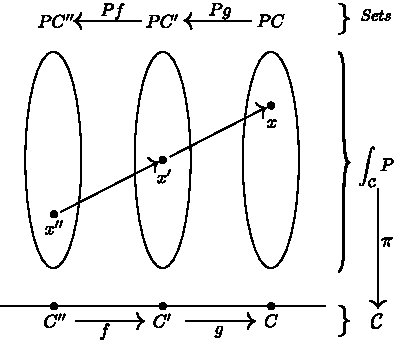
\includegraphics[width=0.8\columnwidth]{fig/catofel.pdf}
\caption{The category of elements of a presheaf functor. Adapted from \cite{Awodey2006}.}
\label{fig:catofel}
\end{figure}

\subsection{Topological deconstruction and synthesis of biological information}

In order to be able to represent objects and their interactions in the global category of higher-order interacting biological entities in terms of diagrams modeled in the local category of such we make use of a generalized form of topology that can be applied to any category meeting a couple of constraints and that can be specialized to, for example, the case in which objects and morphisms of the category take on a particular type of algebraic structure. The purpose of this construction is to develop a method of defining a {\it covering system} composed of interacting entities in the category representing local interactions that can be used to establish a decomposition of objects in the category representing global interactions that may each rely on a certain type of composition of local interactions with respect to any biological system. We first give a conceptual overview of the standard concepts of {\it sieve}, {\it Grothendieck topology}, {\it site}, and {\it sheaf} for an arbitrary category $\cC$ and then explain how sieves on $\mathcal{L}_0$ can be used to specify a topology, and thus a site and sheaves on $\mathcal{L}_1$ under certain conditions.

\iftoggle{thmsty}{
\begin{definition}
\label{definition-sieve}
}{}
For any category $\cC$ and $c \in \Ob(\cC)$ a {\it sieve} $S$ on $c$ is a collection in $\Mor(\cC)$ with codomain $c$ such that for $f,g \in \Mor(\cC)$
$$
f \in S \Rightarrow f \circ g \in S
$$
whenever there is a $g \in \Mor(\cC)$ such that $cod(g)=dom(f)$. Any sieve can be restricted to a sieve on the domain of a map whose codomain is the object of the sieve. If $S$ is a sieve on $c$ and $h:d \rightarrow c \in \Mor(\cC)$ with $cod(h)=c$ then
$$
h^* (S) \equiv \{ g \, | \, cod(g)=d, h \circ g \in S \}
$$
is a sieve on $d$.
\iftoggle{thmsty}{
\end{definition}
}

\begin{figure}
\noindent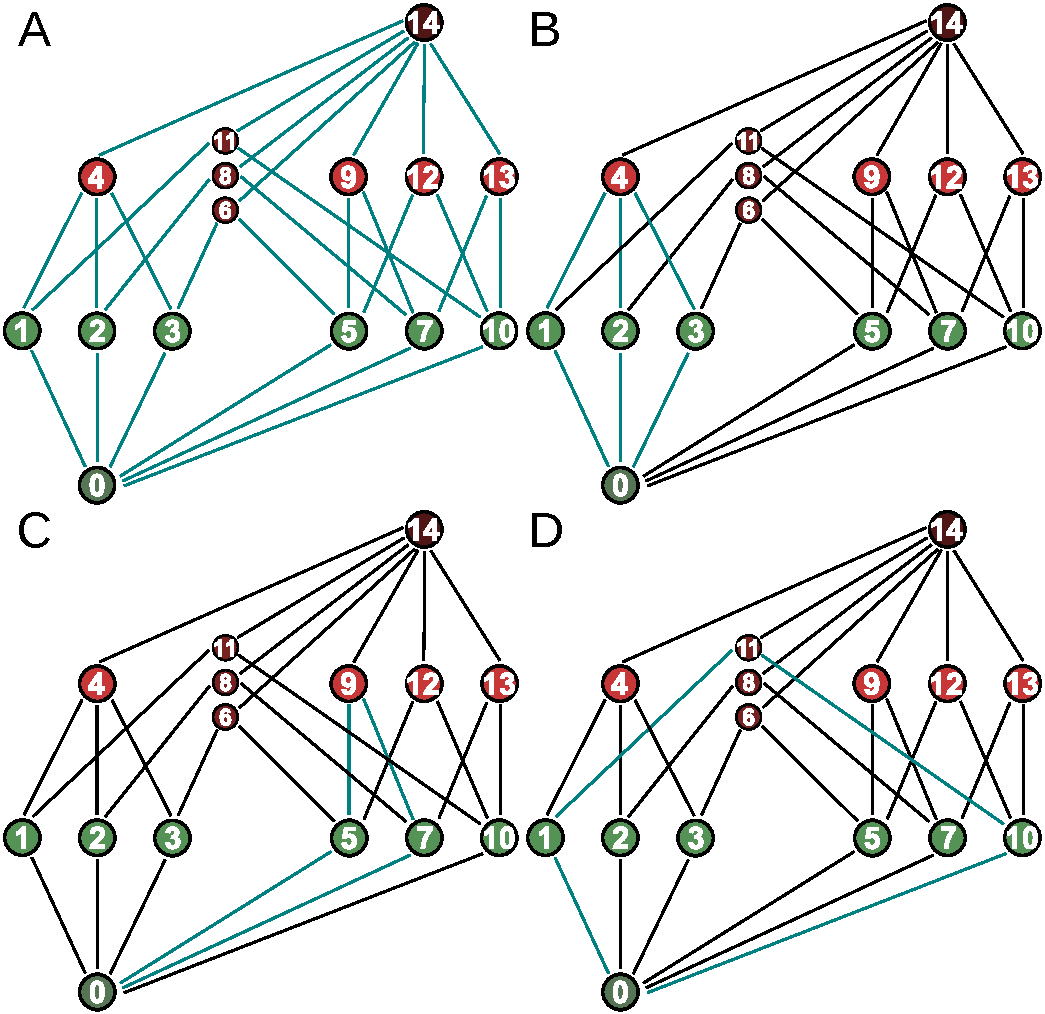
\includegraphics[width=0.8\columnwidth]{fig/sieveHasseSetPartitions4.pdf}
\caption{Sieves conceptualized on {\it Hasse diagrams} of an algebraic lattice. All edges are directed from bottom to top. Blue edges are part of a sieve on an object represented by a node in the lattice. Black edges are part of the lattice but not part of the sieve under consideration. (A) shows the maximal sieve on the lattice, which is equivalent to a sieve on object 14. (B) shows a sieve on object 4, (C) shows a sieve on object 9 and (D) shows a sieve on object 11.}
\label{fig:sieve}
\end{figure}

A sieve is thus a collection of all the morphisms impinging on a given object upon which it is defined. Examples of sieves on an algebraic lattice are shown in figure \ref{fig:sieve}. There is a simple connection between sieves and the Yoneda embedding $PSh:\cC \rightarrow \textit{Sets}^{\cC^{opp}}$. A sieve is a subfunctor $S \subseteq hom(-,c)$ of the functor in the presheaf category on $\cC$ that is represented by $c \in \Ob(\cC)$. Placing constraints on such sieves enables the definition of an abstract notion of topology on a category.

\iftoggle{thmsty}{
\begin{definition}
\label{definition-grothendieck-topology}
}{}
A {\it Grothendieck topology} on a category $\cC$ is a function $J$ that assigns a collection $J(c)$ of sieves on $c$ to each $c \in \Ob(\cC)$ such that conditions of maximality, stability and transitivity are satisfied respectively
\begin{enumerate}
\item the maximal sieve $M_c = \{f \, | \, cod(f) = c\} \in J(c)$,
\item for $S \in J(c)$, $f^*(S) \in J(d)$ for any $f:d \rightarrow c \in \Mor(\cC)$,
\item for $S \in J(c)$, $R \in J(c)$ for any sieve $R$ on $c$ with $f^* (R) \in J(d)$ for all $f:d \rightarrow c \in S$.
\end{enumerate}
Sieves $S$ in $J(c)$ for an object $c \in \Ob(\cC)$ are referred to as $J-covering$ sieves.
\iftoggle{thmsty}{
\end{definition}
}

\iftoggle{thmsty}{
\begin{definition}
\label{definition-basis}
}{}
A {\it basis} for a topology on a category $\cC$ that has pullbacks is a function $B$ that assigns to each object $c \in \Ob(\cC)$ a collection of families $\{c_i \rightarrow c \}$ of morphisms referred to as {\it covering families} in $B(c)$ such that
\begin{enumerate}
\item every family consisting of a single isomorphism $\{ d \cong c \}$ is a covering family in $B(c)$
\item if $\{f_i:c_i \rightarrow c \}$ is a covering family and $g:d \rightarrow c$ is any morphism in $\Mor(\cC)$ then $\{g^* c_i \rightarrow d \}$ is a covering family in $B(d)$ of $d$, which means that the collection of covering families is stable under pullbacks
\item if $\{f_i : c_i \rightarrow c \}_{i \in I}$ is a covering family and $\{ g_{i,j} : c_{i,j} \rightarrow c_i \}_{j \in J_i}$ then the family of composites $\{ f_i \circ g_{i,j} : c_{i,j} \rightarrow c_i \rightarrow c \}_{i \in I, j \in J_i}$ is a covering family in $B(c)$
\end{enumerate}
\iftoggle{thmsty}{
\end{definition}
}

\iftoggle{thmsty}{
\begin{definition}
\label{definition-site}
}{}
A pair $(\cC,J)$ or $(\cC,B)$ consisting of a category $\cC$ and a Grothendieck topology $J$ on $\cC$ or a basis $B$ for such a topology is referred to as a {\it site}. If $S \in J(c)$, then $S$ is a {\it covering sieve} of $c$. If $B$ is a basis on $\cC$, then $B$ is said to {\it generate} a topology $J$ according to the equivalence between the statements that a sieve $S$ is a $J$-cover and that a sieve $S$ contains an associated $B$-cover
$$
S \in J(c) \Longleftrightarrow \exists Q \in B(c), \,\,\, Q \subseteq S.
$$
\iftoggle{thmsty}{
\end{definition}
}

\iftoggle{thmsty}{
\begin{definition}
\label{definition-sheaves}
}{}
Given a basis for, $B$, or an explicit Grothendieck topology, $J$, on a category $\cC$ we can define necessary conditions in order for presheaves $P$ in the presheaf category $\textit{Sets}^{\cC^{opp}}$ to be sheaves on the site $(\cC,J)$. If in addition to $P$ we have the sieve $S$ that is a cover of an object $c \in \Ob(\cC)$, then we can define a {\it matching family} for $S$ from elements of $P$ as a function assigning to each $f:d \rightarrow c \in S$ an element $x_f \in P(d)$ such that
$$
\forall g:e \rightarrow d \in \Mor(\cC), \,\,\, x_f \cdot g = x_{fg},
$$
where $x_f \cdot g \equiv P(g)(x_f)$ and $fg \in S$. We can further define an {\it almagamation} of a matching family as a single element $x \in P(c)$ such that
$$
\forall f \in S, \,\,\, x \cdot f = x_f,
$$
implying that $P(f)(x)=x_f$ and thus $P(g)(P(f)(x))=x_{fg}$. $P$ is then a {\it sheaf} for $J$ when every matching family for all covers of all objects in $\Ob(\cC)$ have a unique amalgamation. A sieve $S$ on an object $c$ is a subfunctor of the functor represented by $c$ under the Yoneda embedding. This is to say that $S \subseteq h^c = hom(-,c)$. In this case, $P$ is a sheaf if and only if for every covering sieve $S$ on $c$ the inclusion $S \hookrightarrow P$ induces an isomorphism $hom(S,P) \cong hom(h^c,P)$. This can also be expressed as the equalizer
\begin{displaymath}
\xymatrix{
P(c) \ar[r]
&
\prod\limits_{f \in S}
P(dom \, f)
\ar@<1ex>[r]^-{p} \ar@<-1ex>[r]_-{a}
&
\prod\limits_{\substack{f,g \,\,\, f \in S \\ dom \, f=cod \, g}}
P(dom \, g)
}
\end{displaymath}
\noindent for each $c \in \Ob(\cC)$ and each cover $S \in J(c)$. $e$ refers to $e(x)=\{x \cdot f\}_f = \{P(f)(x)\}_f$, $p$ refers to $p( \mathbf{x} )_{f,g} = x_{fg}$, and $a$ refers to $a( \mathbf{x} )_{f,g} = x_f \cdot g$ for $\mathbf{x} = \{ x_f \}_{f \in S}$. Given that the equalizer condition, $p \circ e = a \circ e \Leftrightarrow p=a$, is satisfied for a cover $S$ then $P$ is a sheaf with respect to the cover $S$.

Finally, to express the sheaf condition in terms of a basis $B$ for a topology $J$ generated by $B$ on a category $\cC$ having pullbacks. If $Q = \{ f_i : c_i \rightarrow c \}_{i \in I}$ is a B-cover of $c$ a family of elements $x_i \in P(c_i)(i \in I)$ is a matching family for $Q$ if $ x_i \cdot \pi_{ij}^1 = x_j \cdot \pi_{ij}^2$ for all $i,j \in I$. $\pi^1$ and $\pi^2$ are defined as
\begin{displaymath}
\xymatrix{
c_i \times_c c_j \ar[r]^-{\pi_{ij}^2} \ar[d]_{\pi_{ij}^1} & c_j \ar[d]^{f_j} \\
c_i \ar[r]^{f_i} & c
}
\end{displaymath}
\noindent Now again, a presheaf $P \in \textit{Sets}^{\cC^{opp}}$ is a sheaf for the topology $J$ generated by the basis $B$ if and only if for any cover $\{ f_i : c_i \rightarrow c \}_{i \in I}$ in $B$ any matching family $\{ x_i \}_i$ has a unique amalgamation $x \in P(c)$ such that $x \cdot f_i = x_i$ for all $i \in I$. This condition can also be expressed in terms of a diagram that is an equalizer
\begin{displaymath}
\xymatrix{
P(c) \ar[r]
&
\prod\limits_{i \in I}
P(c_i)
\ar@<1ex>[r]^-{p_1} \ar@<-1ex>[r]_-{p_2}
&
P(c_i \times_c c_j)
}
\end{displaymath}
\noindent The morphism $e$ refers to $e(x) = \{ x \cdot f_i \}_i$, $p_1$ refers to $p_1(\{ x_i \})_{i,j} = x_i \cdot \pi_{ij}^1$, and $p_2$ refers to $p_2(\{x_i\})_{i,j} = x_j \cdot \pi_{ij}^{2}$.
\iftoggle{thmsty}{
\end{definition}
}

\subsection{Coherence constraints on emerging transitions in the hierarchical organization of biological systems}

\section{Conclusion}

%------bibliography---%
\bibliographystyle{unsrt} 
\bibliography{bib/books,bib/papers}
%---------------------%


%-----------------------------------------------%
%                   appendix
%-----------------------------------------------%
\appendix
\section{Category theory}\label{app:CatTh}
\iftoggle{thmsty}{
\begin{definition}
\label{definition-category}
}{}
A {\it category} $\mathcal{C}$ is:
\begin{enumerate}
\item A set of objects $\Ob(\mathcal{C})$.
\item For each pair $x, y \in \Ob(\mathcal{C})$ a set of morphisms
$\Mor_\mathcal{C}(x, y)$.
\item For each triple $x, y, z\in \Ob(\mathcal{C})$ a composition
map $ \Mor_\mathcal{C}(y, z) \times \Mor_\mathcal{C}(x, y)
\to \Mor_\mathcal{C}(x, z) $, denoted $(\phi, \psi) \mapsto
\phi \circ \psi$.
\end{enumerate}
Such that these constraints are satisfied:
\begin{enumerate}
\item For every element $x\in \Ob(\mathcal{C})$ there exists a
morphism $\text{id}_x\in \Mor_\mathcal{C}(x, x)$ such that
$\text{id}_x \circ \phi = \phi$ and $\psi \circ \text{id}_x = \psi $.
\item Composition is associative, i.e., $(\phi \circ \psi) \circ \chi =
\phi \circ ( \psi \circ \chi)$.
\end{enumerate}
\iftoggle{thmsty}{
\end{definition}
}

\iftoggle{thmsty}{
\begin{definition}
\label{definition-functor}
}{}
A {\it functor} $F : \mathcal{A} \to \mathcal{B}$
between two categories $\mathcal{A}, \mathcal{B}$ is:
\begin{enumerate}
\item A map $F : \Ob(\mathcal{A}) \to \Ob(\mathcal{B})$.
\item For every $x, y \in \Ob(\mathcal{A})$ a map
$F : \Mor_\mathcal{A}(x, y) \to \Mor_\mathcal{B}(F(x), F(y))$,
denoted $\phi \mapsto F(\phi)$.
\end{enumerate}
These data should be compatible with composition and identity morphisms
in the following manner: $F(\phi \circ \psi) =
F(\phi) \circ F(\psi)$ for a composable pair $(\phi, \psi)$ of
morphisms of $\mathcal{A}$ and $F(\text{id}_x) = \text{id}_{F(x)}$.
\iftoggle{thmsty}{
\end{definition}
}

\iftoggle{thmsty}{
\begin{definition}
\label{definition-transformation-functors}
}{}
Let $F, G : \mathcal{A} \to \mathcal{B}$ be functors.
A {\it natural transformation}, or a {\it morphism of functors}
$t : F \to G$, is a collection $\{t_x\}_{x\in \Ob(\mathcal{A})}$
such that
\begin{enumerate}
\item $t_x : F(x) \to G(x)$ is a morphism in the category $\mathcal{B}$, and
\item for every morphism $\phi : x \to y$ of $\mathcal{A}$ the following
diagram is commutative
$$
\xymatrix{
F(x) \ar[r]^{t_x} \ar[d]_{F(\phi)} & G(x) \ar[d]^{G(\phi)} \\
F(y) \ar[r]^{t_y} & G(y) }
$$
\end{enumerate}
\iftoggle{thmsty}{
\end{definition}
}

We can define a category having functors as objects and natural transformations as morphisms, which is called a functor category, by recognizing that every functor $F$ comes with the {\it identity} transformation $\text{id}_F : F \to F$. In addition, given a morphism of
functors $t : F \to G$ and a morphism of functors $s : E \to F$
then the {\it composition} $t \circ s$ is defined by the rule
$$
(t \circ s)_x = t_x \circ s_x : E(x) \to G(x)
$$
for $x \in \Ob(\mathcal{A})$.
This is a morphism of functors
from $E$ to $G$.
Thus, given categories
$\mathcal{A}$ and $\mathcal{B}$ we obtain the category of functors between $\mathcal{A}$ and
$\mathcal{B}$.

\iftoggle{thmsty}{
\begin{definition}
\label{definition-equivalence-categories}
}{}
An {\it equivalence of categories}
$F : \mathcal{A} \to \mathcal{B}$ is a functor such that there
exists a functor $G : \mathcal{B} \to \mathcal{A}$ such that
the compositions $F \circ G$ and $G \circ F$ are isomorphic to the
identity functors $\text{id}_\mathcal{B}$,
respectively $\text{id}_\mathcal{A}$.
In this case we say that $G$ is a {\it quasi-inverse} to $F$.
\iftoggle{thmsty}{
\end{definition}
}

\iftoggle{thmsty}{
\begin{definition}
\label{definition-adjoint}
}{}
Let $\mathcal{C}$, $\mathcal{D}$ be categories.
Let $u : \mathcal{C} \to \mathcal{D}$ and
$v : \mathcal{D} \to \mathcal{C}$ be functors.
We say that $u$ is a {\it left adjoint} of $v$ or that
$v$ is a {\it right adjoint} to $u$, written $u \dashv v$, if there are bijections
$$
\phi_{X,Y}:\Mor_\mathcal{D}(u(X), Y)
\simeq
\Mor_\mathcal{C}(X, v(Y))
$$
functorial in $X \in \Ob(\mathcal{C})$, and
$Y \in \Ob(\mathcal{D})$.
\iftoggle{thmsty}{
\end{definition}
}

Morphisms that are associated with each other according to the bijections of an adjunction are called {\it adjoint transposes} of one another. If $g:u(X) \rightarrow Y$, $g \in \Mor(\cD)$ then $g^*: X \rightarrow v(Y)$, $g^* \in \Mor(\cC)$ is given by $\phi_{X,Y}(g) = g^*$. Similarly for $f: X \rightarrow v(Y)$, $f \in \Mor(\cC)$ with $f^*:u(X) \rightarrow Y$, $f^* \in \Mor(\cD)$ is given by $\phi_{X,Y}^{-1}(f) = f^*$. We see then that $g^* = f$ and $f^* = g$.

\iftoggle{thmsty}{
\begin{definition}
\label{definition-opposite}
}{}
Given a category $\mathcal{C}$ the {\it opposite category}
$\mathcal{C}^{opp}$ is the category with the same objects
as $\mathcal{C}$ but all morphisms reversed.
\iftoggle{thmsty}{
\end{definition}
}

\iftoggle{thmsty}{
\begin{definition}
\label{definition-contravariant}
}{}
Let $\mathcal{C}$, $\mathcal{S}$ be categories.
A {\it contravariant} functor $F$
from $\mathcal{C}$ to $\mathcal{S}$
is a functor $\mathcal{C}^{opp}\to \mathcal{S}$.
\iftoggle{thmsty}{
\end{definition}
}

\iftoggle{thmsty}{
\begin{definition}
\label{definition-presheaf}
}{}
Let $\mathcal{C}$ be a category.
\begin{enumerate}
\item A {\it presheaf of sets on $\mathcal{C}$}
or simply a {\it presheaf} is a contravariant functor
$F$ from $\mathcal{C}$ to $\textit{Sets}$. When $F$ is a covariant functor $F : \mathcal{C}^{opp} \rightarrow \textit{Sets}$.
\item The category of presheaves is denoted $\textit{PSh}(\mathcal{C})$.
\end{enumerate}
\iftoggle{thmsty}{
\end{definition}
}

\iftoggle{thmsty}{
\begin{definition}
\label{definition-products}
}{}

Let $x, y\in \Ob(\mathcal{C})$,
A {\it product} of $x$ and $y$ is
an object $x \times y \in \Ob(\mathcal{C})$
together with morphisms
$p\in \Mor_{\mathcal C}(x \times y, x)$ and
$q\in\Mor_{\mathcal C}(x \times y, y)$ such
that the following universal property holds: for
any $w\in \Ob(\mathcal{C})$ and morphisms
$\alpha \in \Mor_{\mathcal C}(w, x)$ and
$\beta \in \Mor_\mathcal{C}(w, y)$
there is a unique
$\gamma\in \Mor_{\mathcal C}(w, x \times y)$ making
the diagram
$$
\xymatrix{
w \ar[rrrd]^\beta \ar@{-->}[rrd]_\gamma \ar[rrdd]_\alpha & & \\
& & x \times y \ar[d]_p \ar[r]_q & z \\
& & x &
}
$$
commute.
\iftoggle{thmsty}{
\end{definition}
}

\iftoggle{thmsty}{
\begin{definition}
\label{definition-has-products-of-pairs}
}{}
We say the category $\mathcal{C}$ {\it has products of pairs
of objects} if a product $x \times y$
exists for any $x, y \in \Ob(\mathcal{C})$.
\iftoggle{thmsty}{
\end{definition}
}

\iftoggle{thmsty}{
\begin{definition}
\label{definition-coproducts}
}{}
Let $x, y \in \Ob(\mathcal{C})$,
A {\it coproduct}, or {\it amalgamated sum} of $x$ and $y$ is
an object $x \amalg y \in \Ob(\mathcal{C})$
together with morphisms
$i \in \Mor_{\mathcal C}(x, x \amalg y)$ and
$j \in \Mor_{\mathcal C}(y, x \amalg y)$ such
that the following universal property holds: for
any $w \in \Ob(\mathcal{C})$ and morphisms
$\alpha \in \Mor_{\mathcal C}(x, w)$ and
$\beta \in \Mor_\mathcal{C}(y, w)$
there is a unique
$\gamma \in \Mor_{\mathcal C}(x \amalg y, w)$ making
the diagram
$$
\xymatrix{
& y \ar[d]^j \ar[rrdd]^\beta \\
x \ar[r]^i \ar[rrrd]_\alpha & x \amalg y \ar@{-->}[rrd]^\gamma \\
& & & w
}
$$
commute.
\iftoggle{thmsty}{
\end{definition}
}

\iftoggle{thmsty}{
\begin{definition}
\label{definition-has-coproducts-of-pairs}
}{}
We say the category $\mathcal{C}$ {\it has coproducts of pairs
of objects} if a coproduct $x \amalg y$
exists for any $x, y \in \Ob(\mathcal{C})$.
\iftoggle{thmsty}{
\end{definition}
}

\iftoggle{thmsty}{
\begin{definition}
\label{definition-product-category}
}{}
Let $\mathcal{A}$, $\mathcal{B}$ be categories.
The {\it product category} is the category
$\mathcal{A} \times \mathcal{B}$ with
objects
$\Ob(\mathcal{A} \times \mathcal{B}) =
\Ob(\mathcal{A}) \times \Ob(\mathcal{B})$
and
$$
\Mor_{\mathcal{A} \times \mathcal{B}}((x, y), (x', y'))
:=
\Mor_\mathcal{A}(x, x')\times
\Mor_\mathcal{B}(y, y').
$$
Composition of morphisms is defined according to components.
\iftoggle{thmsty}{
\end{definition}
}

\iftoggle{thmsty}{
\begin{definition}
\label{definition-bifunctor}
}{}
Given categories $\mathcal{C}_1$, $\mathcal{C}_2$, and $\mathcal{D}$. A {\it bifunctor} or binary functor or 2-ary functor or functor of two variables, $F$, is a functor whose domain is the product of two categories $F: \mathcal{C}_1 \times \mathcal{C}_2 \rightarrow \mathcal{D}$.
\iftoggle{thmsty}{
\end{definition}
}

\iftoggle{thmsty}{
\begin{definition}
\label{definition-hom-functor}
}{}
The {\it hom-functor} is a bifunctor defined on the product of a category $\mathcal{C}$ with its self-dual category $\mathcal{C}^{opp}$, which takes values in the category $\textit{Sets}$. Thus for a category $C$ its hom-functor is 
$$
hom(-,-): \mathcal{C}^{opp} \times \mathcal{C} \rightarrow \textit{Sets},
$$
which can be curried in two ways
\begin{eqnarray*}
hom^{(-)} &:& \mathcal{C}^{opp} \rightarrow \textit{Sets}^{\mathcal{C}},\\
hom_{(-)} &:& \mathcal{C} \rightarrow \textit{Sets}^{\mathcal{C}^{opp}}.
\end{eqnarray*}
The hom-functor maps
\begin{enumerate}
\item objects $(c,c') \in \mathcal{C}^{opp} \times \mathcal{C}$ to the hom-set $\Mor_{\mathcal{C}} (c,c')$, which is the set of morphisms in $\mathcal{C}$ with domain $c$ and codomain $c'$.
\item morphisms 
$$
(f,g):(c,c') \rightarrow (d,d') \in \Mor(\mathcal{C}^{opp} \times \mathcal{C}),
$$
where $f:d \rightarrow c \in \Mor(\mathcal{C})$ and $g:c' \rightarrow d' \in \Mor(\mathcal{C})$, to the set function
\begin{eqnarray*}
\Mor_{\mathcal{C}}(c,c') &\rightarrow& \Mor_{\mathcal{C}}(d,d')\\
(c \rightarrow c') &\mapsto& (d \rightarrow c \rightarrow c' \rightarrow d')
\end{eqnarray*}
\end{enumerate}
\iftoggle{thmsty}{
\end{definition}
}

\iftoggle{thmsty}{
\begin{definition}
\label{definition-representable-functor}
}{}
For a hom-functor $hom(-,-): \mathcal{C}^{opp} \times \mathcal{C} \rightarrow \textit{Sets}$ for $c \in \Ob(\mathcal{C})$ a covariant and contravariant functor can be derived by specializing the hom-functor to morphisms out of or into the object $c$ as
\begin{eqnarray*}
h^c \equiv hom(-,c) &:& \mathcal{C}^{opp} \rightarrow \textit{Sets}\\
h_c \equiv hom(c,-) &:& \mathcal{C} \rightarrow \textit{Sets}.
\end{eqnarray*}
Functors that are isomorphic to $h^c$ or $h_c$ are referred to as {\it corepresentable or representable functors} respectively and $c$ is their {\it representing object}. Note that $h^c \in \Ob(\textit{PSh}(\mathcal{C}))$.
\iftoggle{thmsty}{
\end{definition}
}{}

\begin{figure}
\noindent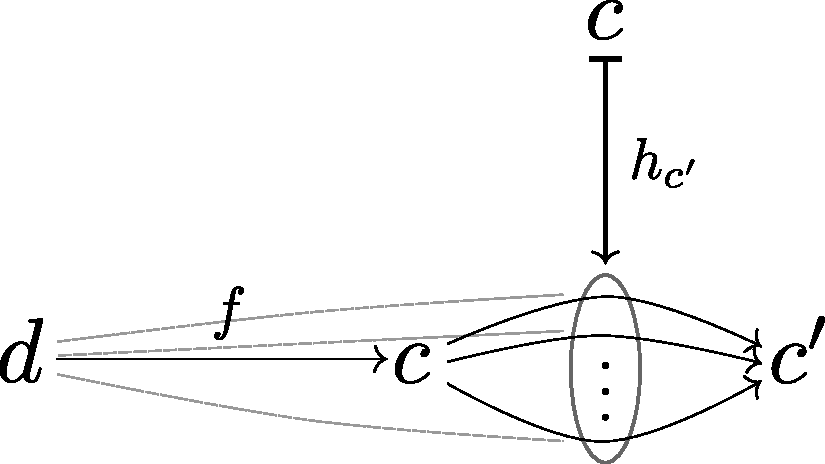
\includegraphics[width=0.7\columnwidth]{fig/hom.pdf}
\caption{The presheaf represented by $c' \in \Ob(\cC)$ is $h^{c'} : \cC^{opp} \rightarrow \textit{Sets}$. It sends objects to the set of morphisms in which they are the domain object with codomain $c'$ and morphisms $f:d \rightarrow c \in \Mor{\cC}$ to set functions $h^{c'} \circ f: \Mor_{\cC}(c,c') \rightarrow \Mor_{\cC}(d,c')$ via pre-composition.}
\label{fig:hom}
\end{figure}

The action of $h^c$ on objects and morphisms is summarized in figure \ref{fig:hom}. The preceding definitions are standard category theoretic constructions. Ellerman has proposed an interpretation of adjoint functors, that demonstrates their relevance to the concept of information encoding and decoding (or sending and receiving) in the context of biological systems \cite{Ellerman2005}.

\iftoggle{thmsty}{
\begin{definition}
\label{definition-birepresentable}
}{}
A bifunctor $bif (-,-): \cC^{opp} \times \cD \rightarrow \textit{Sets}$ is said to be {\it birepresentable} if there exists a pair of functors $F:\cC^{opp} \rightleftarrows \cD:G$ where $c \in \Ob(\cC^{opp})$ and $d \in \Ob(\cD)$ gives
\begin{eqnarray*}
b^{d} \equiv bif(-,d) &:& \mathcal{C}^{opp} \rightarrow \textit{Sets},\\
b_{c} \equiv bif(c,-) &:& \mathcal{D} \rightarrow \textit{Sets}.
\end{eqnarray*}
natural in $c$ and $d$ such that $F \dashv G$. The functors $b^{d}$ and $b_{c}$ are defined on
\begin{enumerate}
\item objects for all $c_i \in \Ob(\cC^{opp})$ and for all $d_i \in \Ob(\cD)$
\begin{eqnarray*}
b^{d} (c_i) &=& \Mor_{\cC^{opp}}(c_i,Gd),\\
b_{c} (d_i) &=& \Mor_{\cD}(Fc,d_i).
\end{eqnarray*}

\item morphisms for all $f_{ij}:c_j \rightarrow c_i \in \Mor(\cC^{opp})$ and for all $g_{ij}:d_i \rightarrow d_j \in \Mor(\cD)$ as
\begin{eqnarray*}
b^{d} (f_{ij}) &:& \Mor_{\cC^{opp}}(c_i,Gd) \rightarrow \Mor_{\cC^{opp}}(c_j,Gd),\\
b_{c} (g_{ij}) &:& \Mor_{\cD}(Fc,d_i) \rightarrow \Mor_{\cD}(Fc,d_j).
\end{eqnarray*}
\end{enumerate}
\iftoggle{thmsty}{
\end{definition}
}

\section{Sieves and sheaves}\label{Sheaves}

\iftoggle{thmsty}{
\begin{definition}
\label{definition-presheaves-injective-surjective}
}{}
Let $\mathcal{C}$ be a category, and let $\varphi : \mathcal{F}
\to \mathcal{G}$ be a map of presheaves of sets.
\begin{enumerate}
\item We say that $\varphi$ is {\it injective} if for every object
$U$ of $\mathcal{C}$ we have $\alpha : \mathcal{F}(U)
\to \mathcal{G}(U)$ is injective.
\item We say that $\varphi$ is {\it surjective} if for every object
$U$ of $\mathcal{C}$ we have $\alpha : \mathcal{F}(U)
\to \mathcal{G}(U)$ is surjective.
\end{enumerate}
\iftoggle{thmsty}{
\end{definition}
}

\iftoggle{thmsty}{
\begin{lemma}
\label{lemma-mono-epi}
}{}
The injective (resp.\ surjective) maps defined above
are exactly the monomorphisms (resp.\ epimorphisms) of
$\textit{PSh}(\mathcal{C})$. A map is an isomorphism
if and only if it is both injective and surjective.
\iftoggle{thmsty}{
\end{lemma}
}{}

\iftoggle{thmsty}{
\begin{definition}
\label{definition-sub-presheaf}
}{}
We say $\mathcal{F}$ is a {\it subpresheaf} of $\mathcal{G}$
if for every object $U \in \Ob(\mathcal{C})$ the set
$\mathcal{F}(U)$ is a subset of $\mathcal{G}(U)$, compatibly
with the restriction mappings.
\iftoggle{thmsty}{
\end{definition}
}

\noindent
In other words, the inclusion
maps $\mathcal{F}(U) \to \mathcal{G}(U)$
glue together to give an (injective) morphism of
presheaves $\mathcal{F} \to \mathcal{G}$.

\iftoggle{thmsty}{
\begin{lemma}
\label{lemma-image}
}{}
Let $\mathcal{C}$ be a category.
Suppose that $\varphi : \mathcal{F} \to \mathcal{G}$ is a
morphism of presheaves of sets on $\mathcal{C}$.
There exists a unique subpresheaf $\mathcal{G}' \subset \mathcal{G}$
such that $\varphi$ factors as
$\mathcal{F} \to \mathcal{G}' \to \mathcal{G}$
and such that the first map is surjective. We
say that $\mathcal{G}'$ is the {\it image of $\varphi$}.
\iftoggle{thmsty}{
\end{lemma}
}

\iftoggle{thmsty}{
\begin{definition}
\label{definition-sieve-s}
}{}
Let $\mathcal{C}$ be a category. Let $U \in \Ob(\mathcal{C})$.
A {\it sieve $S$ on $U$} is a subpresheaf $S \subset h_U$.
\iftoggle{thmsty}{
\end{definition}
}

\noindent
In other words, a sieve on $U$ picks out for each object
$T \in \Ob(\mathcal{C})$ a subset $S(T)$ of the set
of all morphisms $T \to U$. In fact, the only condition
on the collection of subsets
$S(T) \subset h_U(T) = \Mor_\mathcal{C}(T, U)$
is the following rule
\begin{equation}
\label{equation-property-sieve}
\left.
\begin{matrix}
(\alpha : T \to U) \in S(T) \\
g : T' \to T
\end{matrix}
\right\} \Rightarrow
(\alpha \circ g : T' \to U) \in S(T')
\end{equation}

\iftoggle{thmsty}{
\begin{lemma}
\label{lemma-sieves-set}
}{}
Let $\mathcal{C}$ be a category. Let $U \in \Ob(\mathcal{C})$.
\begin{enumerate}
\item The collection of sieves on $U$ is a set.
\item Inclusion defines a partial ordering on this set.
\item Unions and intersections of sieves are sieves.
\item
\label{item-sieve-generated}
Given a family of morphisms $\{U_i \to U\}_{i\in I}$
of $\mathcal{C}$ with target $U$
there exists a unique smallest sieve $S$ on $U$ such that
each $U_i \to U$ belongs to $S(U_i)$.
\item The sieve $S = h_U$ is the maximal sieve.
\item The empty subpresheaf is the minimal sieve.
\end{enumerate}
\iftoggle{thmsty}{
\end{lemma}
}

\iftoggle{thmsty}{
\begin{proof}
}{}
By our definition of subpresheaf, the collection of
all subpresheaves of a presheaf $\mathcal{F}$ is a subset of
$\prod_{U \in \Ob(\mathcal{C})} \mathcal{P}(\mathcal{F}(U))$.
And this is a set. (Here $\mathcal{P}(A)$ denotes
the powerset of $A$.) Hence the collection of sieves on $U$
is a set.

\medskip\noindent
The partial ordering is defined by: $S \leq S'$ if and only if
$S(T) \subset S'(T)$ for all $T \to U$. Notation: $S \subset S'$.

\medskip\noindent
Given a collection of sieves $S_i$, $i \in I$ on $U$ we can
define $\bigcup S_i$ as the sieve with values
$(\bigcup S_i)(T) = \bigcup S_i(T)$ for all
$T \in \Ob(\mathcal{C})$.
We define the intersection $\bigcap S_i$ in the same way.

\medskip\noindent
Given $\{U_i \to U\}_{i\in I}$ as in the statement, consider
the morphisms of presheaves $h_{U_i} \to h_U$. We simply
define $S$ as the union of the images of these maps of presheaves.
\iftoggle{thmsty}{
\end{proof}
}

\iftoggle{thmsty}{
\begin{definition}
\label{definition-sieve-generated}
}{}
Let $\mathcal{C}$ be a category.
Given a family of morphisms $\{f_i : U_i \to U\}_{i\in I}$
of $\mathcal{C}$ with target $U$ we say the sieve
$S$ on $U$ is the {\it sieve  on $U$
generated by the morphisms $f_i$}.
\iftoggle{thmsty}{
\end{definition}
}


\iftoggle{thmsty}{
\begin{definition}
\label{definition-pullback-sieve}
}{}
Let $\mathcal{C}$ be a category.
Let $f : V \to U$ be a morphism of $\mathcal{C}$.
Let $S \subset h_U$ be a sieve. We define the
{\it pullback of $S$ by $f$} to be the sieve
$S \times_U V$ of $V$ defined by the rule
$$
(\alpha : T \to V) \in (S \times_U V)(T)
\Leftrightarrow
(f \circ \alpha : T \to U) \in S(T)
$$
\iftoggle{thmsty}{
\end{definition}
}

$S \times_U V$ can also be referred to as the {\it base change}
of $S$ by $f : V \to U$.

\iftoggle{thmsty}{
\begin{lemma}
\label{lemma-pullback-sieve-section}
}{}
Let $\mathcal{C}$ be a category.
Let $U \in \Ob(\mathcal{C})$.
Let $S$ be a sieve on $U$.
If $f : V \to U$ is in $S$, then
$S \times_U V = h_V$ is maximal.
\iftoggle{thmsty}{
\end{lemma}
}

\iftoggle{thmsty}{
\begin{definition}
\label{definition-topology}
}{}
Let $\mathcal{C}$ be a category.
A {\it topology on $\mathcal{C}$} is given by the following
datum:
\begin{list}{}{}
\item For every $U \in \Ob(\mathcal{C})$
a subset $J(U)$ of the set of all sieves on $U$.
\end{list}
These sets $J(U)$ have to satisfy the following
conditions
\begin{enumerate}
\item For every morphism $f : V \to U$ in $\mathcal{C}$, and
every element $S \in J(U)$ the pullback $S \times_U V$
is an element of $J(V)$.
\item If $S$ and $S'$ are sieves on $U \in \Ob(\mathcal{C})$,
if $S \in J(U)$, and if for all $f \in S(V)$ the pullback
$S' \times_U V$ belongs to $J(V)$, then $S'$ belongs to $J(U)$.
\item For every $U \in \Ob(\mathcal{C})$ the
maximal sieve $S = h_U$ belongs to $J(U)$.
\end{enumerate}
\iftoggle{thmsty}{
\end{definition}
}

\noindent
In this case, the sieves belonging to $J(U)$ are called
the {\it covering sieves}. 

\iftoggle{thmsty}{
\begin{definition}
\label{definition-family-morphisms-fixed-target}
}{}
Let $\mathcal{C}$ be a category.
A {\it family of morphisms with fixed target} in $\mathcal{C}$ is
given by an object $U \in \Ob(\mathcal{C})$, a set $I$ and
for each $i\in I$ a morphism $U_i \to U$ of $\mathcal{C}$ with target $U$.
We use the notation $\{U_i \to U\}_{i\in I}$ to indicate this.
\iftoggle{thmsty}{
\end{definition}
}

\noindent This
notation is meant to suggest an open covering as in topology.

\iftoggle{thmsty}{
\begin{definition}
\label{definition-site-s}
}{}
A {\it site} is given by a category $\mathcal{C}$ and a set
$\text{Cov}(\mathcal{C})$ of families of morphisms with fixed target
$\{U_i \to U\}_{i \in I}$, called {\it coverings of $\mathcal{C}$},
satisfying the following axioms
\begin{enumerate}
\item If $V \to U$ is an isomorphism then $\{V \to U\} \in
\text{Cov}(\mathcal{C})$.
\item If $\{U_i \to U\}_{i\in I} \in \text{Cov}(\mathcal{C})$ and for each
$i$ we have $\{V_{ij} \to U_i\}_{j\in J_i} \in \text{Cov}(\mathcal{C})$, then
$\{V_{ij} \to U\}_{i \in I, j\in J_i} \in \text{Cov}(\mathcal{C})$.
\item If $\{U_i \to U\}_{i\in I}\in \text{Cov}(\mathcal{C})$
and $V \to U$ is a morphism of $\mathcal{C}$ then $U_i \times_U V$
exists for all $i$ and
$\{U_i \times_U V \to V \}_{i\in I} \in \text{Cov}(\mathcal{C})$.
\end{enumerate}
\iftoggle{thmsty}{
\end{definition}
}

We can now define what a sheaf is in two different ways.

\iftoggle{thmsty}{
\begin{definition}
\label{definition-sheaf-sets}
}{}
Let $\mathcal{C}$ be a site, and let $\mathcal{F}$ be a presheaf of sets
on $\mathcal{C}$. We say $\mathcal{F}$ is a {\it sheaf} if
for every covering $\{U_i \to U\}_{i \in I} \in \text{Cov}(\mathcal{C})$
the diagram
\begin{equation}
\label{equation-sheaf-condition}
\xymatrix{
\mathcal{F}(U) \ar[r]
&
\prod\nolimits_{i\in I}
\mathcal{F}(U_i)
\ar@<1ex>[r]^-{\text{pr}_0^*} \ar@<-1ex>[r]_-{\text{pr}_1^*}
&
\prod\nolimits_{(i_0, i_1) \in I \times I}
\mathcal{F}(U_{i_0} \times_U U_{i_1})
}
\end{equation}
represents the first arrow as the equalizer of $\text{pr}_0^*$
and $\text{pr}_1^*$.
\iftoggle{thmsty}{
\end{definition}
}

\iftoggle{thmsty}{
\begin{definition}
\label{definition-sheaf-sets-topology}
}{}
Let $\mathcal{C}$ be a category endowed with a
topology $J$. Let $\mathcal{F}$ be a presheaf of sets
on $\mathcal{C}$.
We say that $\mathcal{F}$ is a
{\it sheaf} on $\mathcal{C}$
if for every $U \in \Ob(\mathcal{C})$ and for
every covering sieve $S$ of $U$ the canonical map
$$
\Mor_{\textit{PSh}(\mathcal{C})}(h_U, \mathcal{F})
\longrightarrow
\Mor_{\textit{PSh}(\mathcal{C})}(S, \mathcal{F})
$$
is bijective.
\iftoggle{thmsty}{
\end{definition}
}

\noindent
The left hand side of the formula equals $\mathcal{F}(U)$ according to the Yoneda lemma. In other words, $\mathcal{F}$ is a sheaf if and only if a section of $\mathcal{F}$
over $U$ is the same thing as a compatible collection of sections
$s_{T, \alpha} \in \mathcal{F}(T)$ parametrized by $(\alpha : T \to U) \in S(T)$, and this for every covering sieve $S$ on $U$.

\end{document}